\chapter{Planung}

\section{Vorgehen}

\subsection{Zeitplanung}

\subsection{GANTT-Diagramm}

\section{Soll-Zustand}

\section{Netzplan}

Die Sensoren sind an den Sensorknoten angeschlossen. Die Daten werden per WLAN
an die Zentraleinheit gesendet. Dort werden die Daten in die Datenbank
geschrieben.\\
Der Webserver greift auf die Datenbank zu und stellt die Daten auf einer Website
übersichtlich dar. (\nameref{Darstellung_Umgebung})

\begin{figure} [htb]
\begin{centering}
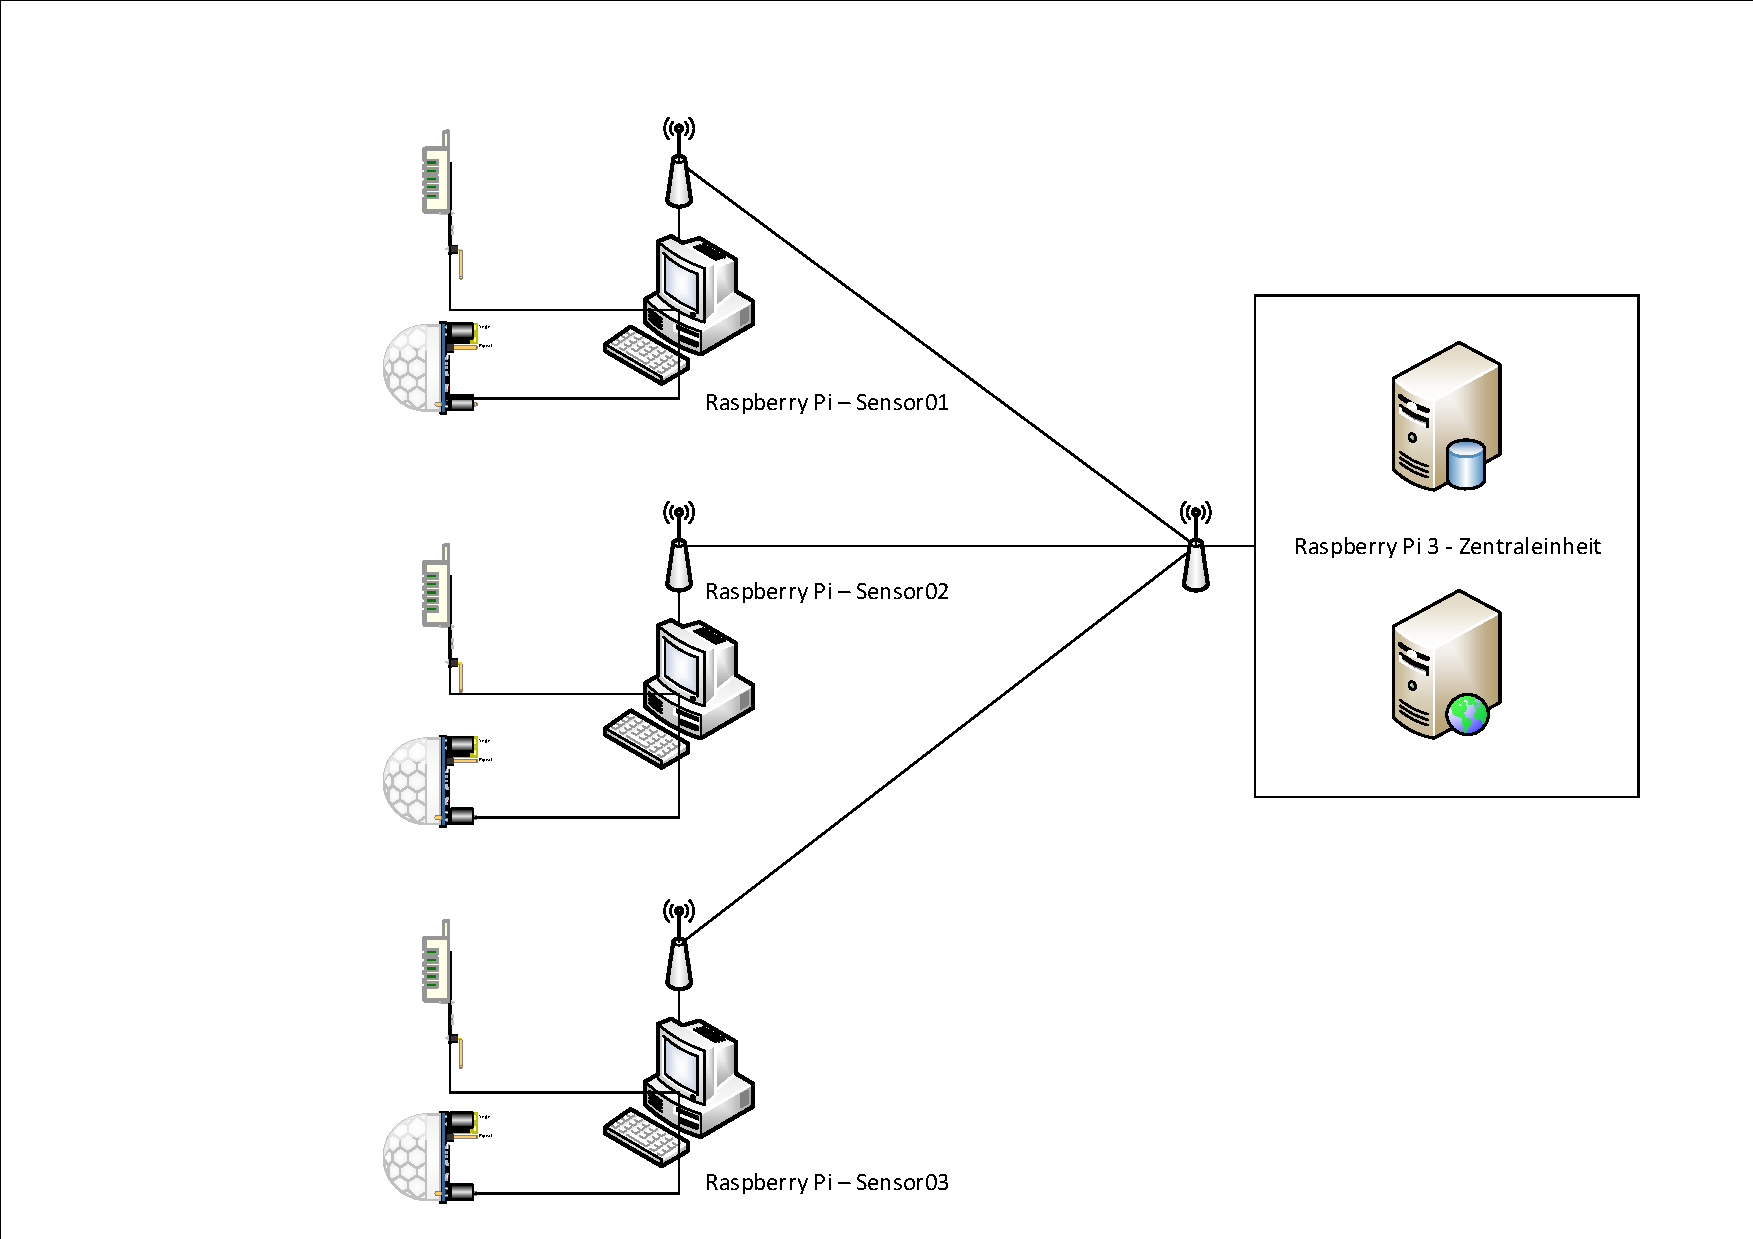
\includegraphics[scale=0.4]{Bilder/Netzplan.pdf}
\caption[Schematische Darstellung der geplanten Umgebung]{Schematische
Darstellung der geplanten Umgebung}
\label{Darstellung_Umgebung}
\end{centering}
\end{figure} 

\section{Datendiagramme}

